%
% File naaclhlt2010.tex
%
% Contact: nasmith@cs.cmu.edu

\documentclass[11pt,letterpaper]{article}
\usepackage{naaclhlt2010}
\usepackage{times}
\usepackage{latexsym}
\usepackage{enumerate}
\usepackage{graphicx}
\setlength\titlebox{6.5cm}    % Expanding the titlebox

\title{Exploring the SVM-KNN with Vision Problems}

\author{Joon Hyuck Choi\\
  The Johns Hopkins University\\
  3400 N Charles Street\\
  Baltimore, MD 21218, USA\\
  {\tt jchoi100@jhu.edu}
  \And
  Joo Chang Lee \\
  The Johns Hopkins University \\
  3400 N Charles Street\\
  Baltimore, MD 21218, USA\\
  {\tt jlee381@jhu.edu}}

\date{Dec 10, 2016}

\begin{document}
\maketitle
\begin{abstract}
The k-Nearest Neighbor (KNN) algorithm is a non-parametric method used for classification and regression. In a previous assignment, we implemented the KNN classifier and one of its variants, the distance weighted KNN. We felt the need to take another step from this assignment and explore another type of the KNN algorithm, which is more involved.

The KNN variant that we explore in this work is the SVM-KNN, a KNN algorithm that makes use of a kernel multiclass support vector machine (SVM) as a subprocedure. The nearest neighbor approach in visual recognition problems has proven to work well in the past. However, despite its benefits, the nearest neighbor approach may suffer from high variation due to finite sampling. The incorporation of an SVM can remedy this situation. The SVM-KNN algorithm attempts to use the standard KNN algorithm with a unanimous voting scheme and then turns to a multiclass SVM if a unanimous agreement was not achieved.

Using an SVM can be effective in the neighborhood of a small number of examples and a small number of classes. We tested this algorithm and compared the performance with the standard KNN on two datasets: MNIST and USPS. We also tested for various values of $K$ on both the KNN and SVM-KNN algorithms.

\end{abstract}

\section{Introduction}

Dynamics in college classrooms have changed drastically in the past decade. Just about ten years ago, rarely did students open their laptops in lecture to take notes$-$rarely did professors allow students to open their computers in class. Today, most students take notes using their laptops. Reasons range from the fact that many students these days have bad penmanship, they are used to typing on their computers, or electronic archives are easier to refer to in the future. However, some students still take notes using pen and paper because they can easily draw figures presented in class and get less distracted on their computers. Nevertheless, it is convenient to have electronic notes. As a result, we became interested in exploring optical character recognition (OCR). We chose to focus on one of the most basic problems in OCR: handwritten digit recognition.

\section{Background}

Performance on visual category recognition has improved by great amounts in the past decade. However, many algorithms are still far from reaching human level performance or are too slow to train. From positive results that past works in the literature have acheived in visual category recognition including the USPS zip code dataset by [5] and shape context based distance on the MNIST dataset [2], the authors of the original paper [1] concluded that exploring other approaches using the nearest neighbhor algorithm could yield fast and accurate results.

The motivations behind using the nearest neighbor approach in visual cateogry recognition are as follow. First, the nearest neighbor approach does not require the explicit construction of a feature space. Second, the nearest neighbor algorithm solves a multiclass classification naturally. Third, as the sample size grows large, the error rate of a nearest neighbor algorithm grows very low.

However, because we are given a limited amount of sample data, the nearest neighbhor algorithm may suffer from high variation. The incorporation of an SVM mitigates this problem. First, the SVM allows for the use of various distance functions. Second, with the finite neighborhood passed by the KNN classifier as input, an SVM trains faster and performs multiclass classification more naturally than it would when given the entire dataset as input. Lastly, the authors of the original paper note that the motivation also came from human pyschophysics. Humans first perform quick coarse categorization and then perform more accurate and slower discrimination with time when performing visual recognition tasks. The KNN works as the preliminary pruning process, and the SVM performs the fine discrimination stage.

\section{Datasets}

For this project, we mainly used two datasets: MNIST and USPS, both of which are datasets of handwritten digits.

\subsection{MNIST \footnote{http://yann.lecun.com/exdb/mnist/}}

MNIST (Mixed National Institute of Standards and Technology database) is a database of handwritten digits commonly used for training image processing systems. The dataset was created by mixing and normalizing the samples from NIST's original datasets. The dataset contains 60,000 training images and 10,000 testing images. Each image is of size 28x28. Currently, the state of the art Convolutional Neural Network approach achieves an error rate of 0.21$\%$ on this dataset [6].

\subsection{USPS \footnote{https://www.otexts.org/1577}}

The USPS dataset is a dataset of handwritten digits with 7,291 training images and 2,007 testing images. The dataset was obtained from the scanning of handwritten digits from envelopes by the U.S. Postal Service. The images in this dataset have been deslanted and size normalized from the original images. Each image is 16x16 grayscale.

\section{SVM-KNN Algorithm [1]}

In this section, we describe the SVM-KNN algorithm. Then we give short overviews of the SVM and KNN algorithms respectively.\\

For input instance $x$,
\begin{enumerate}[(1)]
\item Compute distances of $x$ to all training instances and pick $K$ nearest neighbors.
\item If the $K$ neighbors have the same labels, $x$ is labeled and terminate.\\
\qquad Else, compute the pairwise distances between the $K$ neighbors.
\item Convert the distance matrix to a kernel matrix and apply multiclass SVM.
\item Use resulting classifier to label $x$.
\end{enumerate}

\subsection{Support Vector Machine (SVM)}

Support vector machines are supervised learning models used for classification and regression analysis. Given a set of training instances, each with a corresponding label, an SVM builds a machine learning model that assigns new instances to one category or the other. An SVM is a non-probabilistic classifier. It is a representation of the instances in space, mapped so that the instances of different classes are divided by a gap that is as wide as it can be (max-margin principle). A new instance is mapped into the space and predicted to belong to a class based on the side of the boundary that it falls into. An SVM also allows for non-linear classification with the help of the kernel trick, which implicitly maps inputs into high-dimensional feature spaces. 

\subsection{K-Nearest Neighbors (KNN)}

The K-Nearest Neighbhors Algorithm is a machine learning method used for classification and regression. The input consists of the $K$ nearest training instances in the feature space. In a classification task, the output is a prediction of the class of the given input. The KNN algorithm decides on this prediction by using a majority vote of the input instance's neighbors. The input instance is assigned the label of the class most common among its $K$ neighbors.

\subsection{Implementation}

We based our KNN code from our previous homework assignment. The code in the {\tt predict} function needed the most modification. We needed to take into account the different ways that the USPS and MNIST datasets were encoded from the way the dataset files we were given in class (e.g. {\tt bio.train}). Also, we changed the voting scheme to be unanimous, not majority. In {\tt classify.py}, we needed to modify the {\tt load\textunderscore data} function to be able to correct read and parse the USPS dataset so that it can be readily passed into our methods. Moreover, we needed to adjust the {\tt main} function in this file to correctly handle the two datasets separately.

For the SVM portion of the code, we used {\tt scikit-learn}\footnote{http://scikit-learn.org/stable/modules/svm.html}'s {\tt svm.SVC} with a linear kernel as the kernel. For the tangent distance, XXXXXXXXXXXXXX

The code we wrote can be viewed in our GitHub repository\footnote{https://github.com/jchoi100/machine\textunderscore learning\textunderscore final\textunderscore project}. Run commands are listed in the text file {\tt code/run\textunderscore commands.txt}.

\begin{table}
\begin{center}
\begin{tabular}{|l|r|r|}
\hline \bf K & \bf Accuracy (SVM-KNN) & \bf Accuracy (KNN)\\ \hline
1 & 0.9691 & 0.9691 \\
3 & 0.9721 & \textbf{0.9705} \\
5 & 0.9741 & 0.9688 \\
10 & 0.9764 & 0.9665 \\
30 & 0.9815 & 0.9596 \\
80 & \textbf{0.9831} & 0.9468 \\
110 & 0.9826& N/A \\
150 & 0.9682 & N/A \\
\hline
\end{tabular}
\end{center}
\caption{\label{svm-knn-mnist} SVM-KNN, KNN results on MNIST. }
\end{table}

\begin{table}
\begin{center}
\begin{tabular}{|l|r|r|}
\hline \bf K & \bf Accuracy (SVM-KNN) & \bf Accuracy (KNN)\\ \hline
1 & 0.9437 & 0.9437\\
3 & 0.9467 & \textbf{0.9447}\\
5 & 0.9536 & \textbf{0.9447}\\
10 & \textbf{0.9576} & 0.9357\\
30 & 0.9547 & 0.9118\\
80 & 0.9507 & 0.8764\\
\hline
\end{tabular}
\end{center}
\caption{\label{knn-mnist} SVM-KNN, KNN results on USPS. }
\end{table}

\section{Experimental Results}

We performed experiments in the following ways. We ran the standard KNN algorithm with various $K$ values ($K=1,3,5,10,30,80$) on both MNIST and USPS datasets. We also ran the SVM-KNN algorithm with $K=1,3,5,10,30,80,110,150$ on the two datsets. As an additional experiment, we randomly sampled 7,291 images from the MNIST dataset and ran SVM-KNN to evaluate the difference between MNIST and USPS. (Note that 7,291 is the number of training images in the USPS dataset.) Results and analysis follow in following sections.

\subsection{KNN}

We implemented and ran the standard KNN algorithm on both MNIST and USPS datasets on $K$ values of 1, 3, 5, 10, 30, and 80. Results are shown in the second columns of Table 1 and Table 2.

\subsection{SVM-KNN}

We modified the standard KNN algorithm to use a unanimous voting scheme and integrated scikit-learn's SVM package. For the first part of our experiments, we used a linear kernel and broke ties by choosing the lower index. For the KNN portion of the algorithm, we used $K$ values of 1, 3, 5, 10, 30, 80, 110, and 150. Reasons for using larger $K$ values (110 and 150) are elaborated in the next section. Results are shown in the first columns of Table 1 and Table 2.

In order to compare the MNIST and USPS datasets, we randomly sampled the same number of training images from the MNIST dataset as the USPS dataset contains (7,291 images) and ran the SVM-KNN on this sampled dataset. Results are shown in Table 3.



\subsection{Tangent Distance}

Text

\subsection{RBF Kernel}

Based on the approach taken by the authors in [7], we also ran the SVM-KNN using the RBF kernel on the MNIST dataset.

\section{Discussion}

\subsection{KNN on MNIST and USPS}

We can see from Figures 1 and 2 that as $K$ increases, the accuracy decreases using the standard KNN algorithm. First of all, note that we are not using distance weighted metrics in voting. As the $K$ value increases, the algorithm includes in the neighborhood an increased number of irrelevant samples that are members of different classes. Therefore, these irrelevant, incorrect neighbors disrupt the voting and cause incorrect predictions to take place. Naturally, with more samples in the neighborhood that are further away from our input instance, we get more instances that are not in the same class as our input instance. We get lower accuracy as a result.

We perform slightly better on the MNIST dataset than on the USPS dataset. The authors of the original paper [1] attribute this to the fact that the USPS dataset is naturally harder. The human error rate on the USPS dataset is 2.5$\%$ according to [4]. We empirically verified that this is most likely the case. We discuss more on this thought in Section 6.3.

\begin{figure}[t!]
  \centering
  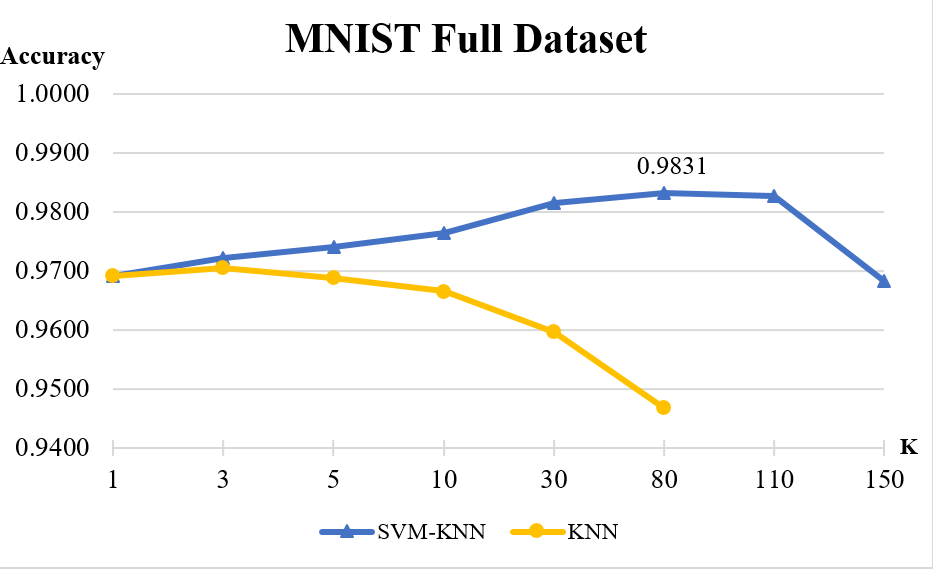
\includegraphics[keepaspectratio, width=0.5\textwidth]{mnist_full.png}
  \caption{Plot of MNIST results.}
\end{figure}

\begin{figure}[t!]
  \centering
  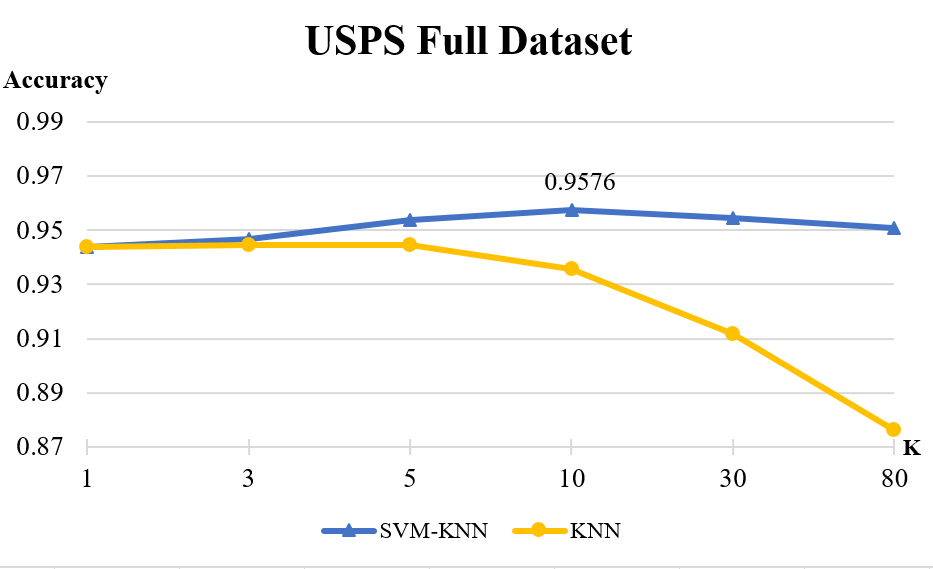
\includegraphics[keepaspectratio, width=0.5\textwidth]{usps_full.png}
  \caption{Plot of USPS results.}
\end{figure}

\begin{table}
\begin{center}
\begin{tabular}{|l|r|r|}
\hline \bf K & \bf Accuracy (SVM-KNN) \\ \hline
1 & 0.9428 \\
3 & 0.9482 \\
5 & 0.9527 \\
10 & 0.9600 \\
30 & 0.9646 \\
80 & 0.9667 \\
110 & \textbf{0.9668} \\
150 & 0.9652 \\
\hline
\end{tabular}
\end{center}
\caption{\label{knn-mnist} Results on MNIST with 7,291 training samples. }
\end{table}

\subsection{SVM-KNN on MNIST and USPS}

In running the SVM-KNN, we can run into three different cases: 1) The KNN algorithm reaches a unanimous vote that is incorrect, and the algorithm outputs that result; 2) The KNN algorithm reaches a unanimous vote that is correct, and the algorithm outputs that result; 3) The KNN algorithm does not agree unanimously and seeks help from the SVM. For the third case, there are four subcases based on the combinations of the KNN majority vote being correct or incorrect and SVM being correct or incorrect. Two of those cases (``KNN majority correct $\rightarrow$ SVM incorrect'' and ``KNN majority incorrect $\rightarrow$ SVM correct'') are of interest to us. The case ``KNN majority correct $\rightarrow$ SVM correct'' is trivial, and the case ``KNN majority incorrect $\rightarrow$ SVM incorrect'' cannot be helped by the SVM-KNN algorithm. This is due to either the limits of this algorithm or the presence of illegible handwriting that caused the human error rates.

We noticed empirically that the first case does not happen very often. It may occur occasionally when the sample image contains messy handwriting. The second case happened most frequently.

The third case was where we saw interesting results. Previously in the KNN experiment, the KNN algorithm reached a majority vote on the wrong classification from time to time. However, in many of those cases, the SVM-KNN algorithm outputted the correct classification nonetheless. For example, for one particular instance, the standard KNN outputted a prediction of ``4'' even though the correct label was ``8'' because the majority of the sample's neighbors were of class ``4''. However, when this sample was run on the SVM-KNN, the algorithm outputted ``8''. We concluded that this was due to the fact that the SVM uses a max-margin principle. Therefore, even though a particular test instance may have many neighbors that are not of the same type, the \textit{max-margin}-ed decision boundary learned by the SVM will correct this error.

However, we also contemplated about the case where the KNN would have been correct by majority vote, but the SVM outputted the wrong classification. We concluded that such cases may happen when our test instance is very close to a support vector on the other side of the decision boundary. Therefore, although the majority of its neighbors are of its own type, SVM may give a wrong prediction.

Furthermore, we noticed that the authors of the original paper provided results for only a single $K$ value for each of the experiments. In particular, they used $K=80$ for SVM-KNN and $K=3$ for KNN on MNIST,  and $K=10$ for SVM-KNN and $K=3$ for KNN on USPS. We decided to run the standard KNN and SVM-KNN on various $K$ values for both datasets. We first tested with $K$ values of 1, 3, 5, 10, 30, 80 for both datasets. We were able to observe a pyramid shaped SVM-KNN accuracy plot for the USPS data with $K=10$ serving as the peak. However, the SVM-KNN accuracy for the MNIST dataset required even larger values of $K$ to observe this \textit{pyramid} behavior. We extended the $K$ testing range to include $K=110$ and $K=150$ to observe declinding accuracy on the MNIST dataset.

We can observe from the SVM-KNN result plots in Figure 1, Figure 2, and Figure 3 that the SVM-KNN accuracy performance increases with larger values of $K$ in the beginning and decreases after a peak at a certain $K$ value. We concluded that the reason the SVM-KNN improves at first is that the SVM can learn with more helpful samples (i.e. neighbors chosen by the KNN algorithm). However, with extremely large values of $K$, the KNN algorithm hands the SVM algorithm a neighborhood with many unhelpful instances that create noise and thus disrupt the SVM from correctly constructing the decision boundary. Therefore, we get higher error rates as $K$ keeps on increasing beyond a certain threshold.
 
\subsection{SVM-KNN on 7,291 Sampled MNIST}

In order to be able to make qualitative comparisons of the MNIST and USPS datasets, we randomly sampled the same number of data points from the MNIST dataset as there are in the USPS dataset. (The MNIST dataset has 60,000 training images while the USPS dataset has only 7,291 training images.) Then, we ran the SVM-KNN algorithm on the reduced, randomly sampled MNIST dataset (call it \textit{MNIST 7291}) and recorded the results. We tested for $K$ values of 1, 3, 5, 10, 30, 80, 110, and 150.

We were able to observe that the MNIST 7291 dataset displayed the \textit{pyramid}-ing behavior at $K=80\dots 110$, which is fairly close to the \textit{pyramid}-ing $K$ value for the full MNIST dataset. Therefore, we were able to see that the size of the training dataset had a small effect in influencing the accuracy of the SVM-KNN on the entire datasets and also on the \textit{pyramid}-ing behavior.

\begin{figure}[t!]
  \centering
  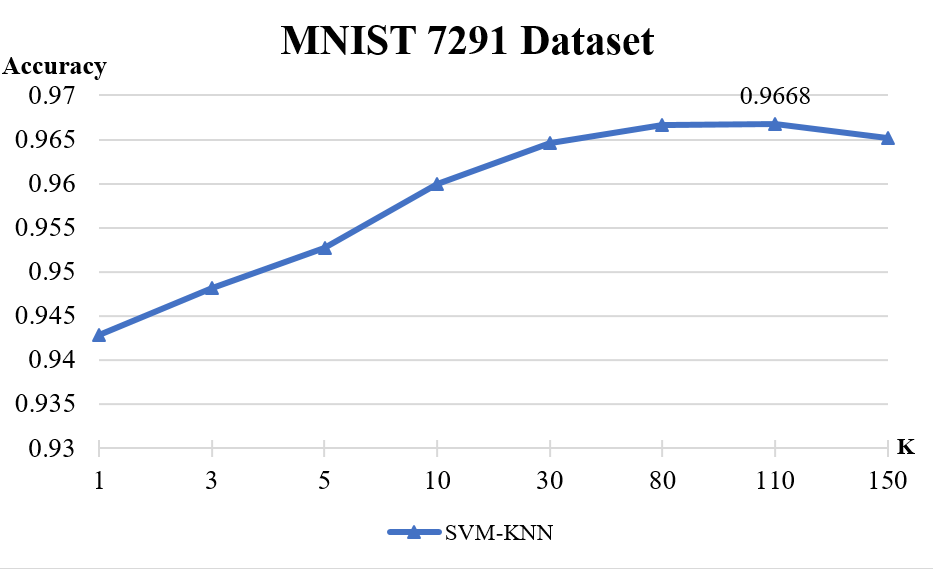
\includegraphics[keepaspectratio, width=0.5\textwidth]{mnist_7291.png}
  \caption{Plot of MNIST 7291 results.}
\end{figure}


\subsection{Tangent Distance SVM-KNN on USPS}

Text

\subsection{RBF Kernel SVM-KNN on MNIST}

Text

\section{Difficulties Faced}

\subsection{Experiment Run Time}

Text

\subsection{Difficulty 2}

Text

\section{Conclusion}

In this project, we explored the SVM-KNN algorithm on several datasets and compared the results with the standard KNN algorithm. We experimented th SVM-KNN and KNN on the MNIST and USPS datasets of handwritten digits on various $K$ values and sample sizes. We conlcude that the standard KNN algorithm performs worse with increasing values of $K$ while the SVM-KNN shows a pyramid-ing behavior with increasing values of $K$. The incorporation of the SVM into the standard KNN algorithm as a subpattern improves the speed and accuracy in visual object recognition tasks for handwritten digit images. Future work needs to explore more on this algorithm's effectiveness on more complex image datasets such as the Caltech 101, Caltech 256, and ImageNet.

\section{Comparison to Proposal}

\subsection{Must Achieve}

\begin{itemize}
\item Create SVM-KNN by using our KNN modified from homework and scikit-learn SVM. $\>\>\>\>\>\>\>\>\>\>\>\>\>\>\>$\textbf{(Done)}
\item Write kernel trick function mentioned. $\>\>\>\>\>\>\>\>\>\>\>\>\>\>\>$\textbf{(Done)}
\item Parse MNIST and USPS datasets to fit as input to our SVM-KNN impelmentation. $\>\>\>\>\>\>\>\>\>\>\>\>\>\>\>$\textbf{(Done)}
\item Run SVM-KNN and KNN on MNIST and USPS using $L_2$ distance function. Try different $K$ values for SVM-KNN and KNN. $\>\>\>\>\>\>\>\>\>\>\>\>\>\>\>$\textbf{(Done)}
\item Compare $\&$ analyze experiment results. $\>\>\>\>\>\>\>\>\>\>\>\>\>\>\>$\textbf{(Done)}
\end{itemize}

\subsection{Expected to Achieve}
\begin{itemize}
\item Use shape contextinstead of $L_2$ to compute distance matrix to feed to Kernel SVM when running SVM-KNN on MNIST. 

\textit{(We were not able to complete this portion because the computations involved were intractable. The authors of the original paper proposed scaling up the input image size from 28x28 to 70x70 on a dataset of 60,000 training images and 10,000 test images.)}
\item Use tangent distance instead of $L_2$ to compute distance matrix to feed to Kernel SVM when running SVM-KNN on USPS.
\end{itemize}

\subsection{Would Like to Achieve}
\begin{itemize}
\item Experiment SVM-KNN on Caltech 101 [3]. 

\textit{(We were not able to XXXXXXXXXXXX)}
\end{itemize}

\subsection{Extra Work Not Mentioned in Proposal}

\begin{itemize}
\item Text

\end{itemize}

\begin{thebibliography}{}

\bibitem[\protect\citename{Zhang, Berg, Maire, Malik}2006]{Zhang, Berg, Maire, Malik:2006}
1. Hao Zhang, Alexander C. Berg, Michael Maire, Jitendra Malik.
\newblock 2006.
\newblock {\em SVM-KNN: Discriminative Nearest Neighbor Classification for Visual Category Recognition}.
\newblock 2006 IEEE Computer Society Conference on Computer Vision and Pattern Recognition.

\bibitem[\protect\citename{Belongie, Malik, Puzicha}2002]{Belongie, Malik, Puzicha:2002}
2. Serge Belongie, Jitendra Malik, Jan Puzicah.
\newblock 2002.
\newblock {\em Shape Matching and Object Recognition Using Shape Contexts}.
\newblock IEEE Trans. Pattern Anal. Mach. Intell.

\bibitem[\protect\citename{Fei-Fi, Fergus, Perona}2004]{Fei-Fi, Fergus, Perona:2004}
3. L. Fei-Fei, R. Fergus and P. Perona.
\newblock 2004.
\newblock {\em SVM-KNN: One-Shot Learning of Object
Categories}.
\newblock 2004 IEEE Trans. Pattern Recognition and Machine Intelligence. In press.

\bibitem[\protect\citename{Bromley, Sackinger}1991]{Bromley, Sackinger:1991}
4. Jane Bromley and Eduard Sackinger.
\newblock 1991.
\newblock {\em Neural-network and K-nearest-neighbor Classifiers}.
\newblock Technical Report 11359-910819-16TM, AT$\&$T.

\bibitem[\protect\citename{Simard, LeCun, Denker}1993]{Simard, LeCun, Denker: 1993}
5. Patrice Simard, Yann LeCun, John Denker.
\newblock 1993.
\newblock {\em Efficient Pattern Recognition Using a New Transformation Distance}.
\newblock In NIPS, pages 50-58, San Francisco, CA, USA. Morgan Kaufmann Publishers Inc.

\bibitem[\protect\citename{Wan, Zeiler, Zhang, LeCun, Fergus}2013]{Wan, Zeiler, Zhang, LeCun, Fergus: 2013}
6. Li Wan, Matthew Zeiler, Sixin Zhang, Yann LeCun, Rob Fergus.
\newblock 2013.
\newblock {\em Regularization of Neural Networks using DropConnect}.
\newblock International Conference on Machine Learning 2013.

\bibitem[\protect\citename{Maji, Malik}2013]{Maji, Malik: 2009}
7. Subhransu Maji, Jitendra Malik.
\newblock 2009.
\newblock {\em Fast and Accurate Digit Classification}.
\newblock EECS Department, University of California, Berkeley, Tech. Rep. UCB/EECS-2009-159.


\end{thebibliography}

\end{document}
